\documentclass[letterpaper, 10 pt, conference]{article} 
\usepackage[english]{babel}
\usepackage{amsmath,amssymb,amscd,amsthm} % variety of useful math macros
\usepackage[inner=1.5 cm, outer = 1.5 cm, top=1 cm, bottom = 1.5 cm]{geometry}
\usepackage{subcaption}
%For inserting graphics
\usepackage{graphicx}
\usepackage[dvipsnames]{xcolor}
\usepackage{listings}
\usepackage[utf8]{inputenc}
\usepackage{hyperref}
\usepackage{array, multirow}
\usepackage{lipsum}
\usepackage{natbib}

\bibliographystyle{abbrvnat}

\newtheorem{thm}{Theorem}
\newtheorem{prop}{Proposition}
\newtheorem{lemma}{Lemma}
\newtheorem{ex}{Exercise}
\newtheorem{defn}{Definition}

\newcommand\ql{\textquotedblleft}
\newcommand\qr{\textquotedblright}


\newcommand\E{\ensuremath{\mathbb{E}}}
\newcommand\N{\ensuremath{\mathbb{N}}}
\renewcommand{\P}{\ensuremath{\mathbb{P}}}
\newcommand\Q{\ensuremath{\mathbb{Q}}}
\newcommand\R{\ensuremath{\mathbb{R}}}
\newcommand\Z{\ensuremath{\mathbb{Z}}}

\newcommand\Om{\ensuremath{\Omega}}
\newcommand{\w}{\ensuremath{\omega}}

\newcommand\var[1]{\, \mathrm{Var} \left( #1 \right)}

\newcommand\pr[1]{\, \mathbb{P} \left( #1 \right)}

\newcommand\cov[1]{\, \mathrm{Cov} \left( #1 \right)}

\newcommand\expec[1]{\, \mathbb{E} \lbrack #1 \rbrack}

\title{Convolutions, variance and covariance
}

\hypersetup{
	colorlinks=true,
	linkcolor=blue,
	filecolor=magenta,      
	urlcolor=blue,
	citecolor=MidnightBlue
}



\lstset{ 
	backgroundcolor=\color{white},   % choose the background color; you must add \usepackage{color} or \usepackage{xcolor}; should come as last argument
	basicstyle=\footnotesize,        % the size of the fonts that are used for the code
	breakatwhitespace=false,         % sets if automatic breaks should only happen at whitespace
	breaklines=true,                 % sets automatic line breaking
	%captionpos=b,                    % sets the caption-position to bottom
	commentstyle=\color{PineGreen},    % comment style
	deletekeywords={...},            % if you want to delete keywords from the given language
	escapeinside={\%*}{*)},          % if you want to add LaTeX within your code
	extendedchars=true,              % lets you use non-ASCII characters; for 8-bits encodings only, does not work with UTF-8
	firstnumber=1,                % start line enumeration with line 1000
	frame=single,	                   % adds a frame around the code
	keepspaces=true,                 % keeps spaces in text, useful for keeping indentation of code (possibly needs columns=flexible)
	keywordstyle=\color{black},       % keyword style
	language=R,                 % the language of the code
	morekeywords={*,...},            % if you want to add more keywords to the set
	numbers=none,                    % where to put the line-numbers; possible values are (none, left, right)
	numbersep=5pt,                   % how far the line-numbers are from the code
	numberstyle=\tiny\color{gray}, % the style that is used for the line-numbers
	rulecolor=\color{black},         % if not set, the frame-color may be changed on line-breaks within not-black text (e.g. comments (green here))
	showspaces=false,                % show spaces everywhere adding particular underscores; it overrides 'showstringspaces'
	showstringspaces=false,          % underline spaces within strings only
	showtabs=false,                  % show tabs within strings adding particular underscores
	stepnumber=2,                    % the step between two line-numbers. If it's 1, each line will be numbered
	stringstyle=\color{purple},     % string literal style
	tabsize=2,	                   % sets default tabsize to 2 spaces
	title=\lstname                   % show the filename of files included with \lstinputlisting; also try caption instead of title
}

\author{G. Palafox}

\begin{document}
\maketitle

\section{Convolutions}
A convolution is, in the more general sense, an operator between two functions which produces a third function. In this section, an application of convolutions of probability functions on finite groups is explored. In particular, convolutions are used to obtain the distribution of a random walk on a finite group. After the basic theory is presented, a practical example is given. Most of what is discussed in this section, and further topics regarding random walks on finite groups, can be found in the books of \citet{Steinberg_2012} or \citet{Diaconis_1988}.
\subsection{Random walks on finite groups}
Let $G$ be a finite group \citep{Herstein_1975}. A probability on $G$ is a function $P : G \longrightarrow [0,1]$  such that 
\begin{equation}
	\sum_{g \in G} P(g) = 1.
\end{equation}
For a subset $A \subseteq G$, one defines $P(A) := \sum_{g \in A} P(g)$. Now, suppose $P, Q$ are probabilities on $G$, and $X \sim P, \, Y \sim Q$ are chosen independently at random. What is the probability of $XY = g$ for some $g$? If $Y = h$, it must be that $X = gh^{-1}$ for $XY$ to occur. Because of independence, the probability of this happening is $P(gh^{-1}) Q(h)$. Summing the probabilities over all possible $h$ gives us the probability of $XY = g$ equal to
\begin{equation}
	\sum_{h \in G} P(gh^{-1}) Q(h) = P \ast Q (g),
\end{equation}
where $\ast$ denotes the convolution operator. Thus, if $X, \, Y$ are independent and $X \sim P, Y \sim Q$, it follows that $XY \sim P \ast Q$. This in turn can be used to model a random walk on $G$ as follows. Starting at the identity $e$ of $G$, a walker chooses $X_1 \in G$ at random according to a probability $P$, and moves to $X_1$. Then, the walker chooses $X_2$ according to $P$ and moves to $X_2 X_1$. Following this process, the walker is choosing a sequence of independent, identically distributed random variables $X_1, X_2, \dots$ with common distribution $P$, landing at $X_k X_{k-1} \cdots X_1$ at step $k$. Let 
\begin{equation}
\delta_g (h) = \begin{cases}
1 & \text{ if } h = g;\\
0 & \text{ if } h \neq g.\\
\end{cases}
\end{equation}
With this notation, one can let $Y_0 \sim \delta_e$ (so $Y_0 = e$ with probability 1), and $Y_k = X_k Y_{k-1}$ for $k \geq 1$. The random variable $Y_k$ gives the position of the walker in the $k$-th step, and by the preceding discussion, $Y_k \sim P^{\ast k}$, where $P^{\ast k}$ denotes the convolution of $P$ with itself $k$ times.  

\subsubsection{Ehrenfest's urn}
For a concrete example, the following is given. Suppose there are two urns, $A$ and $B$, and $n$ balls. At time 0, all balls are in urn $A$. At each step, one ball is chosen uniformly at random, and moved to the other urn. Denote by $\Z/2\Z$ the group of integers modulo 2. The state at step $t$ can be encoded in a vector $v = (c_1, \dots, c_n) \in (\Z / 2 \Z)^n$, where $c_i = 0$ if and only if ball $i$ is in urn $A$. Denote by $e_i$ the element of $ (\Z / 2 \Z)^n $ having a 1 in its $i$-th coordinate, and 0 in the rest. If at an arbitrary time the state of the process is encoded by a vector $v$ as previously described, changing ball $i$ to a different urn consists of adding $e_i$ to the state vector $v$. That is, the state changes to $v + e_i$. Thus, starting at identity $e = (0, 0, \dots, 0)$ (all balls in urn $A$), the process of interchanging balls between the urns corresponds to a random walk on $(\Z / 2 \Z)^n$ driven by probability
\begin{equation}
P(g) = \begin{cases}
1/n & \text{ if } g \in \lbrace e_1, e_2, \dots, e_n\rbrace;\\
0 & \text{ else.}\\
\end{cases}
\end{equation}
%
A thousand steps of this process, with fifty balls total, was simulated with R \citep{R} on a Jupyter notebook \citep{jupyter}. The average amount of balls in urns $A$ and $B$ where 25.25 and 24.75 respectively, which suggests the urns are balanced on average. Histograms showing the distribution of the balls in the urns are shown in Figure \ref{fig:hist_urns}. Additionally, using ImageMagick \citep{imagemagick}, a GIF animation\footnote{The notebook with the code for all the simulations in this report, as well the GIF animation, can be found in the Github Repository: \url{https://github.com/palafox794/AppliedProbabilityModels/tree/master/Assignment11}.}  was created for twenty steps of this process with six balls total.

\begin{figure}
	\centering
	\begin{subfigure}{0.45\linewidth}
		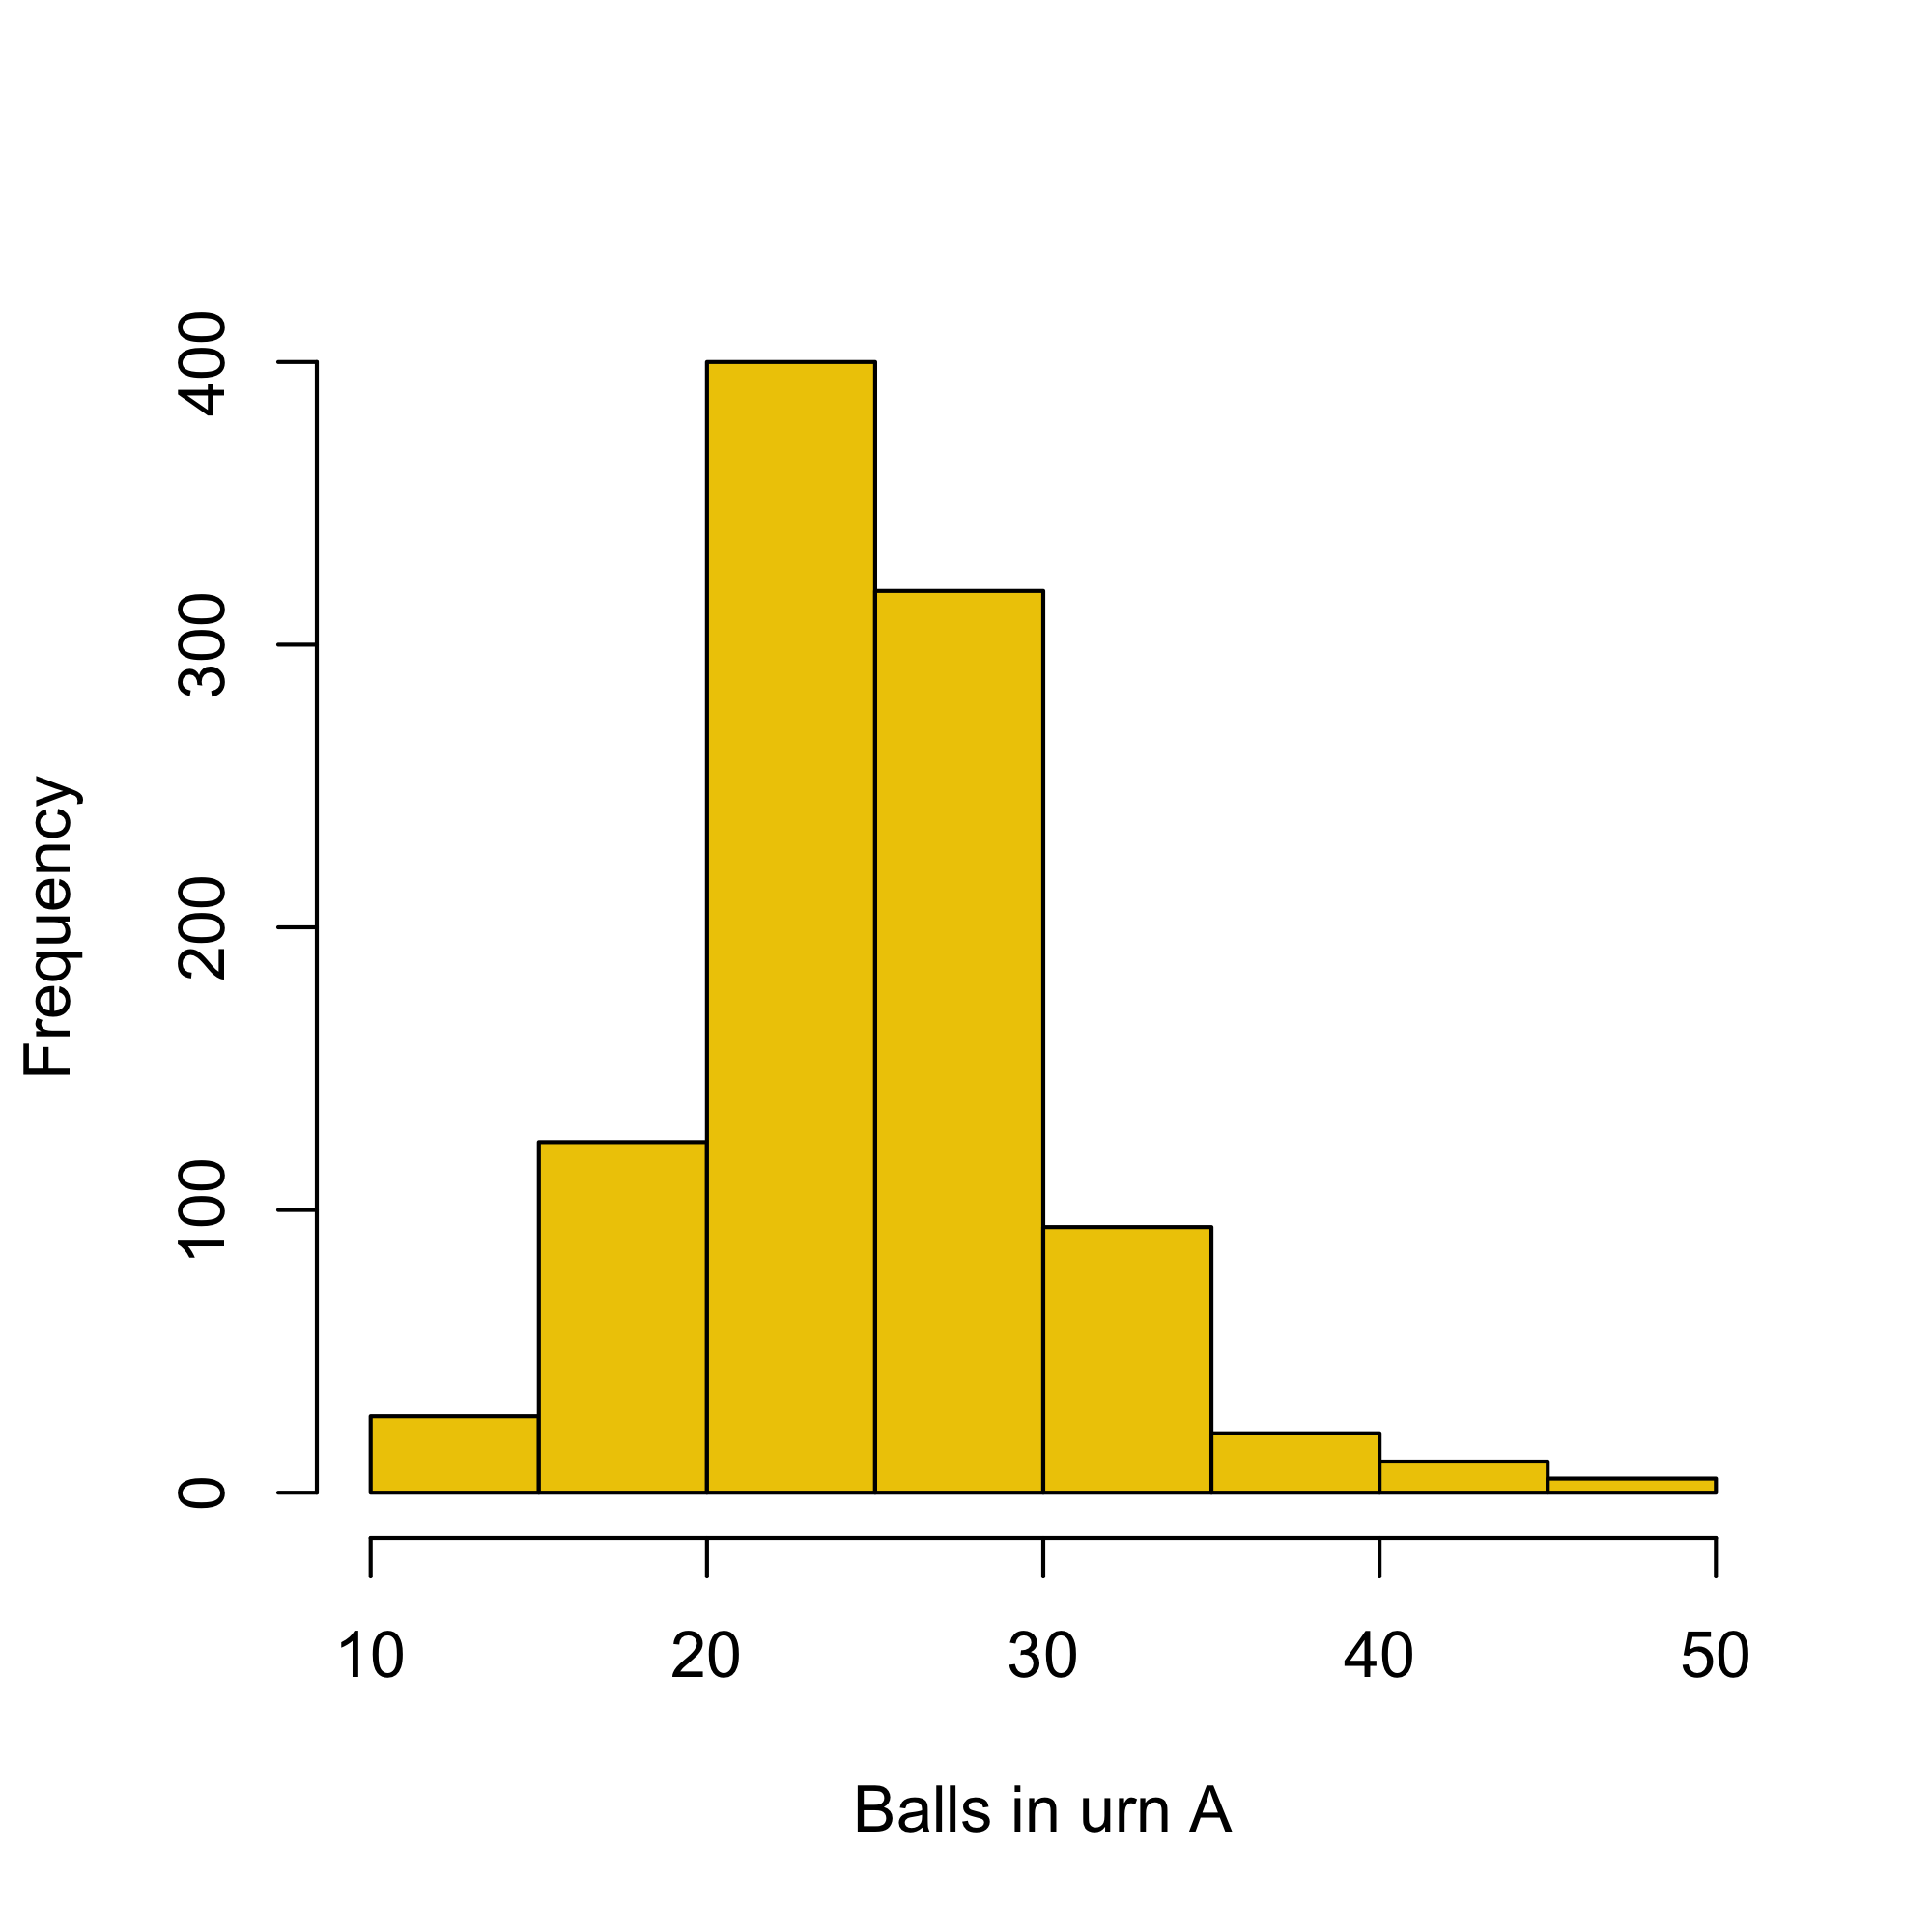
\includegraphics[width=\linewidth]{hist_urnA}
		\caption{Distribution of balls in urn $A$.}
		\label{fig:hist_urnA}
	\end{subfigure}
	\hfill
	\begin{subfigure}{0.45\linewidth}
		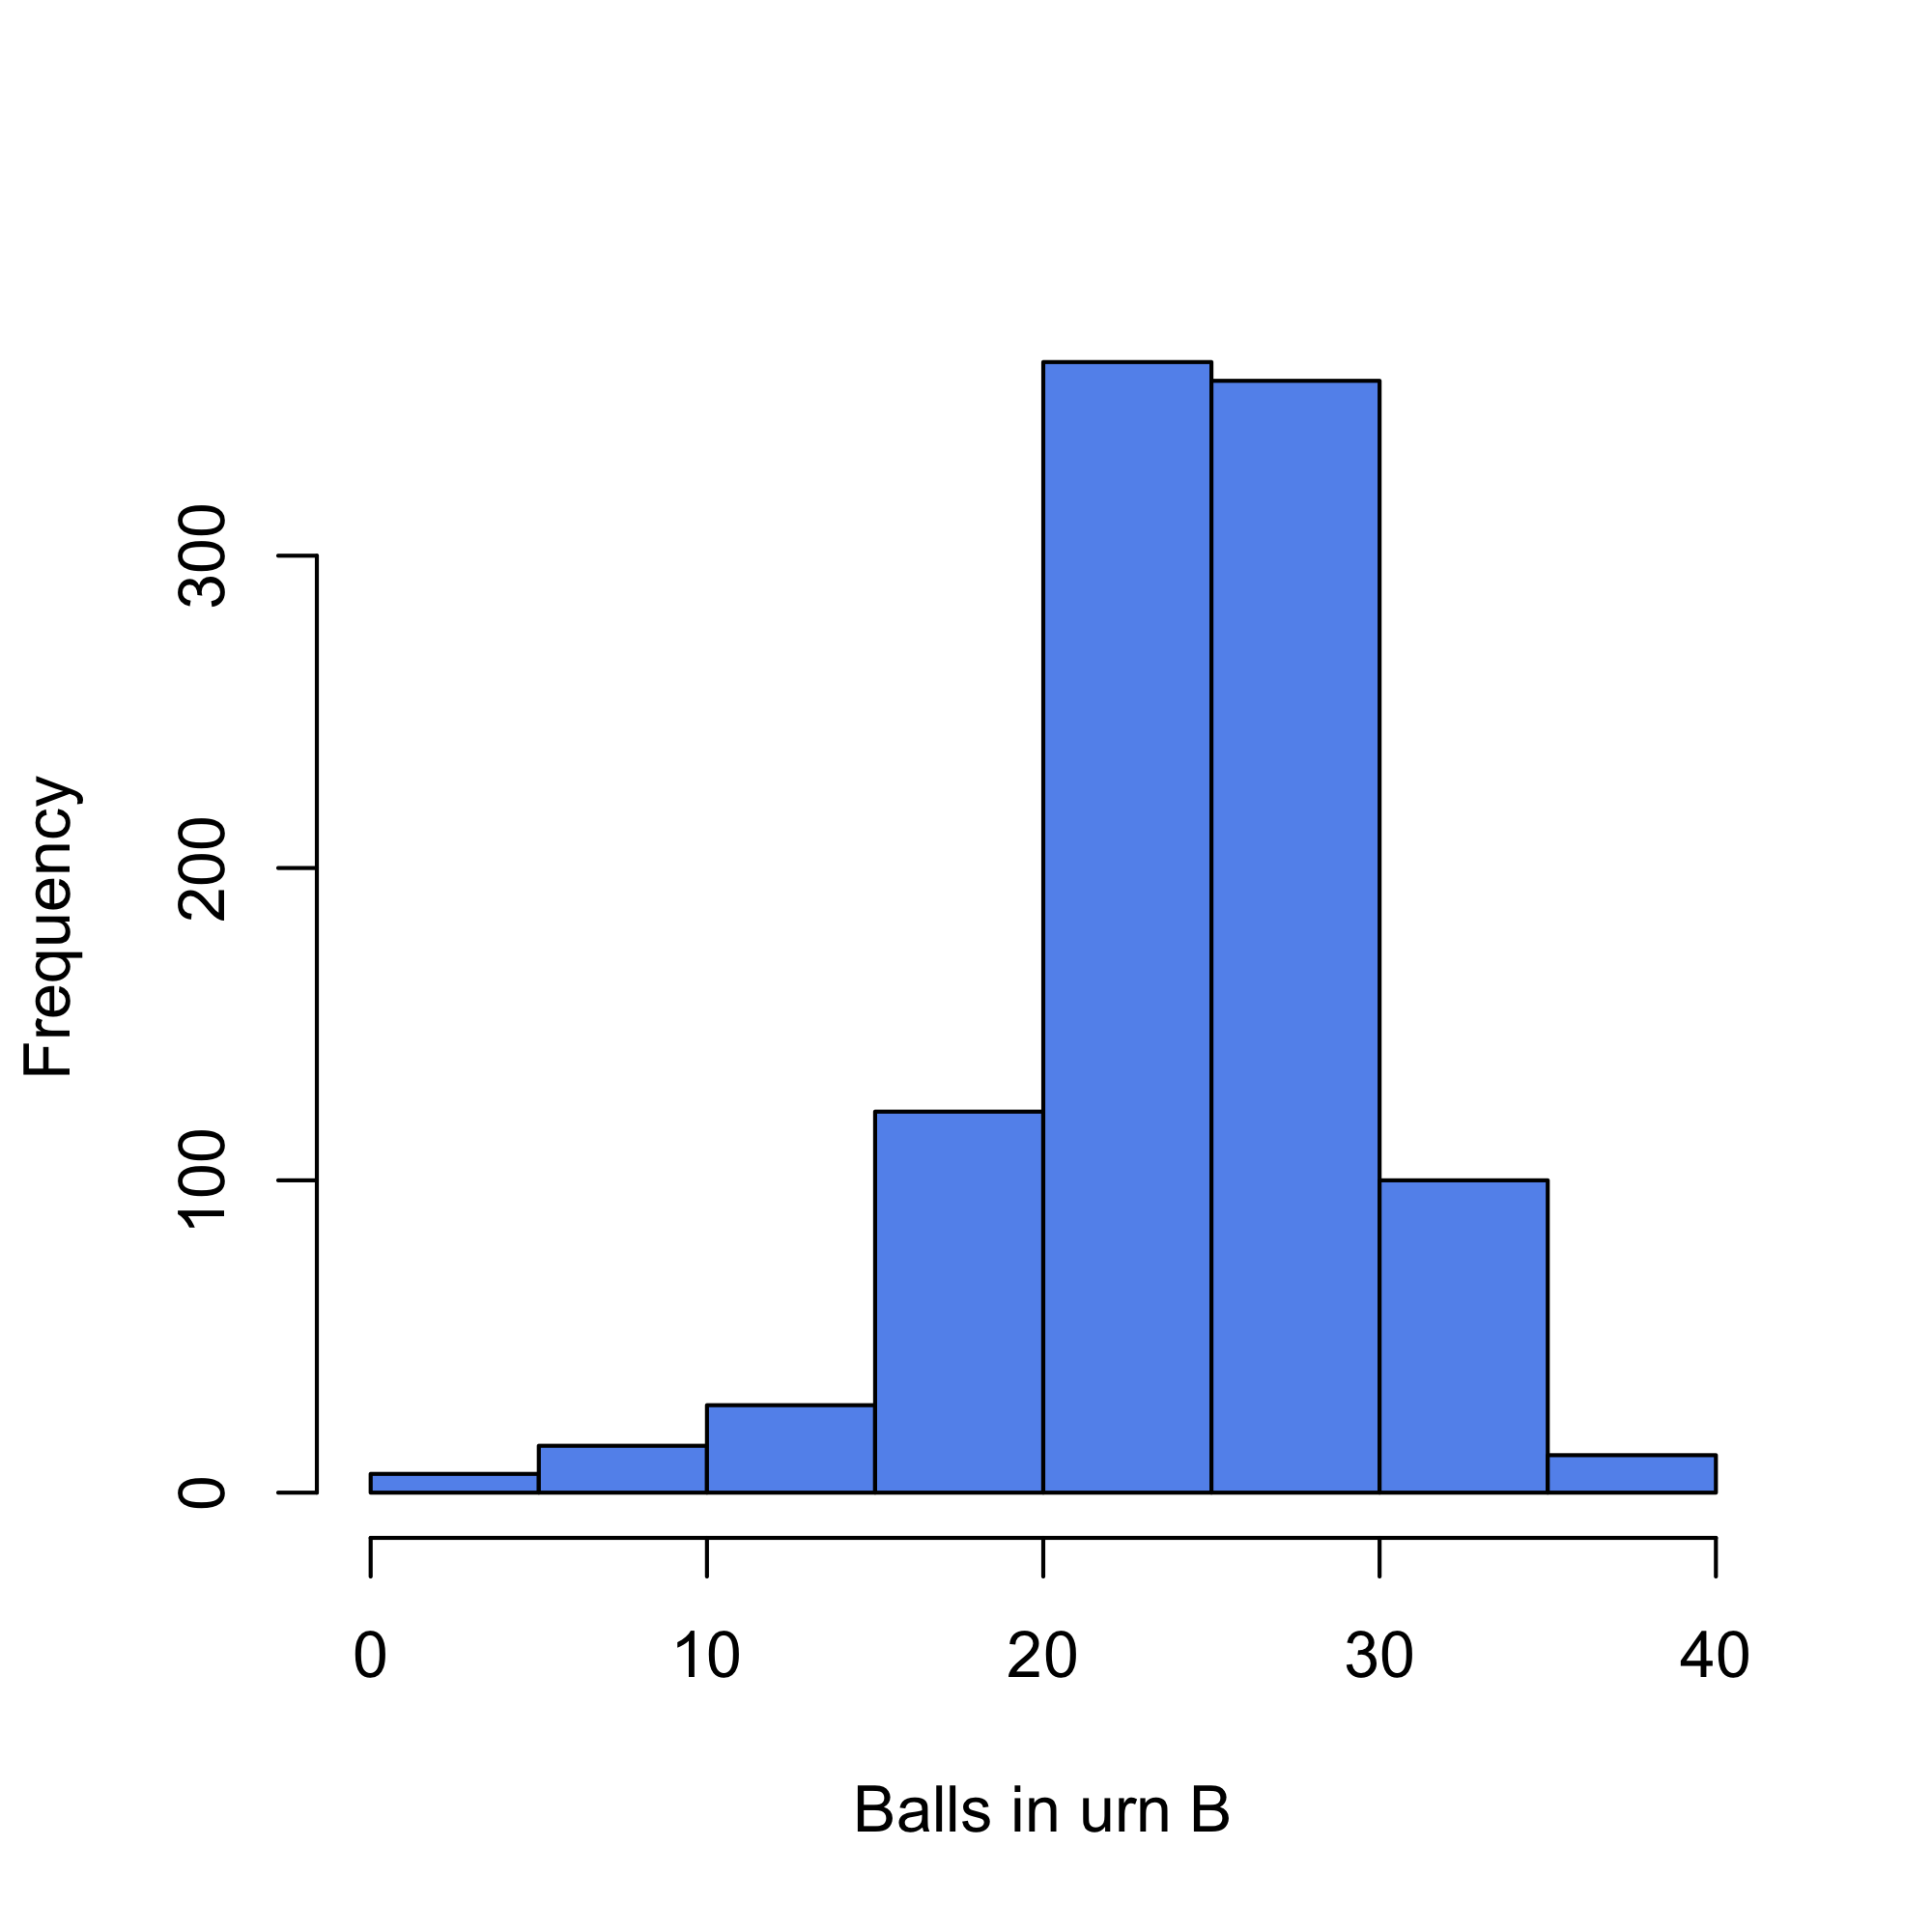
\includegraphics[width=\linewidth]{hist_urnB}
		\caption{Distribution of balls in urn $B$.}
		\label{fig:hist_urnB}
	\end{subfigure}
	\caption{Histogram for ball distribution in a thousand steps of an Erhenfest process with fifty balls.} 
	\label{fig:hist_urns}
\end{figure}
\section{Goodness of fit}
In this section, we perform a goodness of fit test to determine whether the degree distribution of Pennsylvania's road network \citep{snapnets} follows a Poisson distribution. The network has $|V| = 1,088,092$ nodes, and an average degree of $\lambda_d = 2.834$. A $\chi^2$ goodness of fit test is performed to see if the road \ql is random\qr. Given the large size of the road, if nodes were connected to each other at random, a Poisson degree distribution would be expected \citep{Newman_2018}. To perform the test, first the nodes of degree $k = 1, 2, \dots, 14$ are counted. Then, the expected Poisson distribution is obtained computationally, generating $|V|$ numbers following a $\mathrm{Poiss}(\lambda_d)$ distribution. The expected and observed degrees are displayed in Table \ref{tab:deg_exp_obs}. Writing $O_k$ for the observed nodes with degree $k$, and $E_k$ for the expected nodes with degree $k$, a statistic  
\begin{equation}
	\sum_{k = 1}^{14} = \frac{(O_i - E_i)^2}{E_i} =  672,672.24.
\end{equation}
 is obtained. The corresponding $p$-value is 0, so it is concluded that the degree distribution is not Poisson. 
 
% latex table generated in R 4.0.0 by xtable 1.8-4 package
% Thu Nov 12 19:57:31 2020
\begin{table}
	\centering
	\caption{Observed and expected degree of nodes.}
	\begin{tabular}{rrr}
		\hline
		Degree & Expected & Observed \\ 
		\hline
		1 & 245,208 & 188,317 \\ 
		2 & 256,577 & 90,740 \\ 
		3 & 243,159 & 532,686 \\ 
		4 & 171,512 & 267,256 \\ 
		5 & 97,772 & 7,759 \\ 
		6 & 45,727 & 1,237 \\ 
		7 & 18,825 &  80 \\ 
		8 & 6,526 &  13 \\ 
		9 & 2,039 &   4 \\ 
		10 & 550 &   0 \\ 
		11 & 147 &   0 \\ 
		12 &  41 &   0 \\ 
		13 &   7 &   0 \\ 
		14 &   2 &   0 \\ 
		\hline
	\end{tabular}
	\label{tab:deg_exp_obs}
\end{table}

\section{Theoretical results}
To conclude this work, two theorems concerning variance and covariance are presented. Theorem \ref{thm:cov} was tested computationally for random integers $a, b, c, d$ between one and two hundred, and a pair of one thousand number pseudo-random vectors $X, Y$, where  $X \sim \mathrm{Unif}(0,1), Y \sim \mathrm{Exp}(0.5)$; $X \sim N(0,1), Y \sim \mathrm{Exp}(0.5)$; and $X \sim \mathrm{Geom}(0.33), Y \sim \mathrm{Poiss}(1)$. In a thousand repetitions, the equality always held. Theorem \ref{thm:var} was also verified computationally with the same pair of vectors $X, Y$, and it too held true in each of the one thousand repetitions.

\begin{thm} \label{thm:cov}
	For constants $a, b, c, d$ and random variables $X, Y,$
	\begin{equation}
		\cov{a X + b, c Y + d} = a c  \cov{X, Y}.
	\end{equation}
\end{thm}
\begin{proof}
	By definition, it is seen that
	\begin{align}
		\cov{a X + b, c Y + d} &= \expec{(aX+b)(cY+d)} - \expec{a X + b} \expec{c Y + d}\\
		&= \expec{ac XY + ad   X + bc   Y + bd} - (a \expec{x} + b)(c \expec{y} + d)\\
		&= ac   \expec{XY} + ad   \expec{X} + bc    \expec{Y} + bd - ac   \expec{X} \expec{Y} - ad   \expec{X} - bc   \expec{Y} - bd\\
		&= ac(\expec{XY} - \expec{X} \expec{Y})\\
		&= ac   \cov{X, Y}.
	\end{align}
\end{proof}

\begin{thm}\label{thm:var}
	For random variables $X, Y$, 
	\begin{equation}
		\var{X+Y} = \var{X} + \var{Y} + 2   \cov{X, Y}.
	\end{equation}
\end{thm}
\begin{proof}
	Since $\var{X} = \expec{X^2} - \expec{X}^2$, it follows that
	\begin{align}
		\var{X+Y} &= \expec{(X+Y)^2} - \expec{X+Y}^2 \\
		&= \expec{X^2 + 2 X Y + Y^2} - (\expec{X} + \expec{Y} )^2 \\
		&= \textcolor{Maroon}{\expec{X^2}} + 2 \expec{XY} + \textcolor{MidnightBlue}{\expec{Y^2} } \textcolor{Maroon}{ - \expec{X}^2} - 2 \expec{X} \expec{Y} \textcolor{MidnightBlue}{ - \expec{Y}^2} \\
		&= \textcolor{Maroon}{\var{X}} + \textcolor{MidnightBlue}{\var{Y}} + 2( \expec{XY} - \expec{X} \expec{Y} ) \\
		&= \var{X} + \var{Y} + 2 \cov{X, Y}	.	
	\end{align}
\end{proof}

%%%%%%%%%%%%%%%%%%%%%%%%%%%%%%%%%%%%%%%%%%%%%%%%%%%%%%%%%%%%%%%%%%%%%%%%%%%%%%%%

\bibliography{ref}

\end{document}
